\documentclass{article}
\usepackage{amsmath}
\usepackage{geometry}
\geometry{hmargin=2.5cm,vmargin=1.5cm}
\usepackage{graphicx}

\title{L'Accélération Adaptative}
\author{Nouni2}
\date{Juillet 2024}

\begin{document}

\maketitle

\section{Introduction}

L'accélération adaptative (\(a_{\text{adapt}}\)) est une mesure critique pour modéliser le comportement des conducteurs sur les routes. Elle dépend de plusieurs facteurs, dont la distance de sécurité (\(d_{\text{safety}}\)) et les coefficients de sensibilité à la distance et à la vitesse relative (\(k_1\) et \(k_2\)). Cette étude explore en détail comment ces paramètres influencent l'accélération adaptative en tenant compte des autres usagers de la route.

\section{Preuve de la Loi d'Accélération Adaptative}

Pour prouver la loi d'accélération adaptative, considérons d'abord les composants impliqués dans la distance de sécurité (\(d_{\text{safety}}\)) et la distance relative (\(\Delta d\)).

La distance de sécurité est définie comme :
\[
d_{\text{safety}} = v \cdot t_{\text{reaction}} + \frac{v^2}{2a_{\text{deceleration}}}
\]

La distance relative entre les véhicules est :
\[
\Delta d = d - d_{\text{safety}}
\]

L'accélération adaptative (\(a_{\text{adapt}}\)) dépend de la distance relative normalisée par la distance de sécurité et de la vitesse relative entre deux véhicules (\(\Delta v = v_1 - v_2\)) :
\[
a_{\text{adapt}} = k_1 \left( \frac{\Delta d}{d_{\text{safety}}} \right) + k_2 \Delta v
\]

En substituant \(\Delta d\) et \(d_{\text{safety}}\), nous obtenons :
\[
a_{\text{adapt}} = k_1 \left( \frac{d -  v \cdot t_{\text{reaction}} + \frac{v^2}{2a_{\text{deceleration}}} }{v \cdot t_{\text{reaction}} + \frac{v^2}{2a_{\text{deceleration}}}} \right) + k_2 \Delta v
\]

Cela nous donne l'équation fondamentale régissant l'accélération adaptative.


\section{Introduction de la Variabilité des Conducteurs}

Pour modéliser la variabilité du comportement des conducteurs, nous introduisons des coefficients aléatoires \(k_1\) et \(k_2\), ainsi que le temps de réaction \(t_{\text{reaction}}\).

\subsection{Distribution des Coefficients de Sensibilité}

Les coefficients \(k_1\) et \(k_2\) suivent une distribution Beta. La distribution Beta est choisie pour modéliser des variables aléatoires limitées à un intervalle \([0, 1]\) et qui peuvent avoir une grande variété de formes en fonction de ses paramètres :
\[
k_1 \sim \text{Beta}(\alpha_1, \beta_1)
\]
\[
k_2 \sim \text{Beta}(\alpha_2, \beta_2)
\]

La distribution Beta est particulièrement utile pour modéliser des comportements variés dans une population, où certaines valeurs peuvent être plus fréquentes que d'autres, reflétant ainsi la diversité des comportements des conducteurs.

\subsection{Distribution du Temps de Réaction}

Le temps de réaction \(t_{\text{reaction}}\) suit une distribution normale, ce qui est courant pour modéliser des phénomènes naturels où la plupart des valeurs sont proches de la moyenne avec une symétrie autour de cette moyenne :
\[
t_{\text{reaction}} \sim \mathcal{N}(\mu_t, \sigma_t^2)
\]

Cette distribution reflète le fait que la majorité des conducteurs ont un temps de réaction proche de la moyenne, avec quelques-uns ayant des temps de réaction significativement plus courts ou plus longs.

\section{Analyse des Résultats}

La figure ci-dessous montre l'impact de différents paramètres sur l'accélération adaptative, avec un focus particulier sur le temps de réaction.

\begin{figure}[h!]
    \centering
    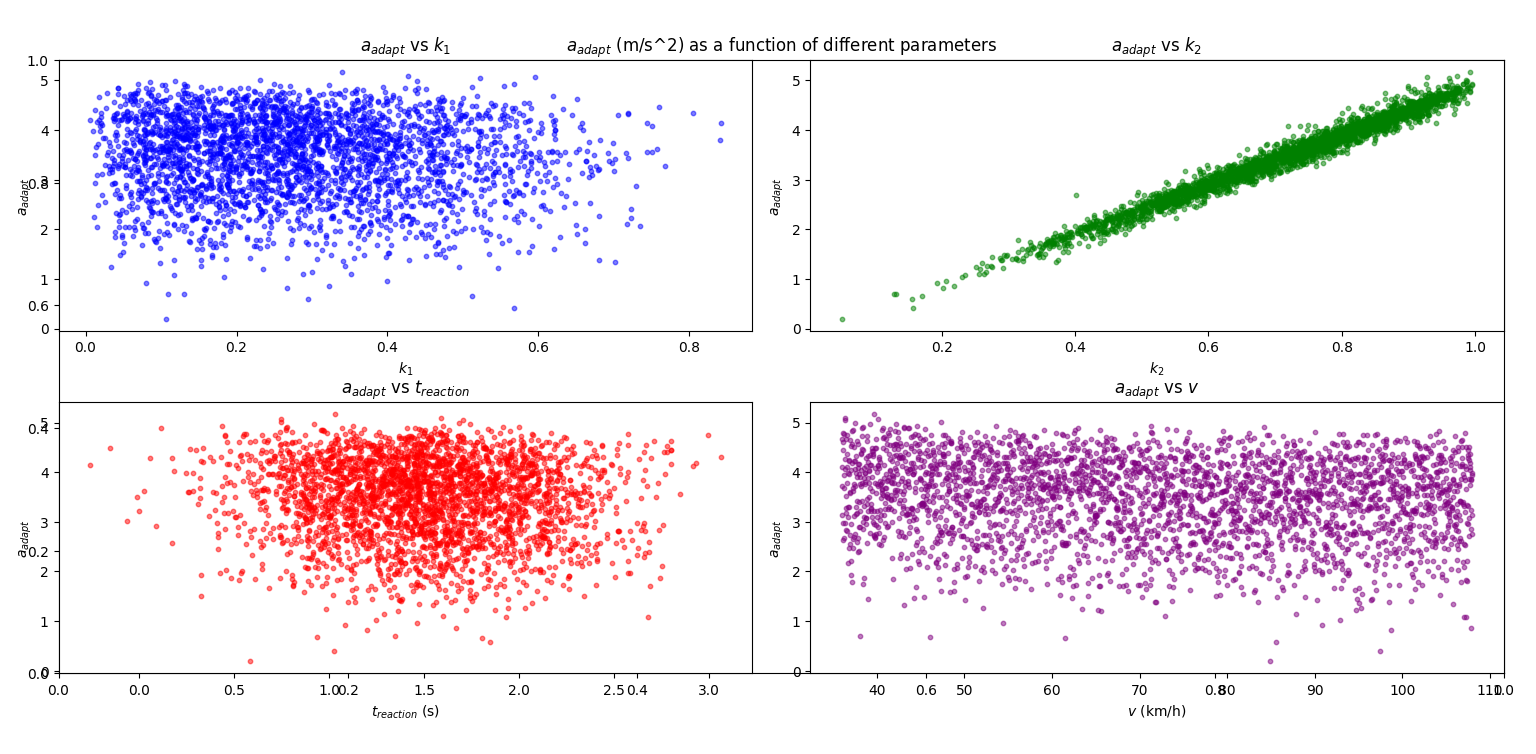
\includegraphics[width=\linewidth]{Adaptative_acceleration.png}
    \caption{\(a_{\text{adapt}}\) en fonction de \(k_1\), \(k_2\), \(t_{\text{reaction}}\) et \(v\)}
    \label{fig:adaptative_acceleration}
\end{figure}

\subsection{Impact du Temps de Réaction (\(t_{\text{reaction}}\))}

Le graphique \(a_{\text{adapt}} \) vs \( t_{\text{reaction}} \) montre une agglomération notable des points autour de la valeur \( t_{\text{reaction}} = 1.5 \) secondes. La majorité des conducteurs ont un temps de réaction moyen d'environ 1.5 secondes, ce qui est conforme aux observations typiques de la psychologie du comportement des conducteurs. À mesure que le temps de réaction s'éloigne de cette valeur centrale, les valeurs de \(a_{\text{adapt}}\) tendent à diminuer de manière symétrique. Cela reflète le fait que les conducteurs avec des temps de réaction plus longs réagissent plus lentement aux changements de la distance de sécurité, entraînant une variabilité plus grande dans \(a_{\text{adapt}}\). Bien que le temps de réaction influence notablement l'accélération adaptative, cette influence est moins prononcée que celle de \(k_2\).

\subsection{Impact du Coefficient de Sensibilité à la Distance (\(k_1\))}

Le graphique \(a_{\text{adapt}} \) vs \( k_1 \) montre une dispersion considérable sans corrélation évidente entre \(k_1\) et \(a_{\text{adapt}}\). Cependant, il y a une agglomération notable des points pour les petites valeurs de \(k_1\), indiquant que la majorité des conducteurs ont un coefficient de sensibilité à la distance \(k_1\) relativement faible. Cela suggère que la distance de sécurité n'est pas le principal facteur d'ajustement de l'accélération pour la plupart des conducteurs. En d'autres termes, la plupart des conducteurs n'ajustent pas leur accélération principalement en fonction de la distance de sécurité, mais d'autres facteurs, comme la vitesse relative, peuvent jouer un rôle plus important.

\subsection{Impact du Coefficient de Sensibilité à la Vitesse Relative (\(k_2\))}

En revanche, le graphique \(a_{\text{adapt}} \) vs \( k_2 \) montre une forte corrélation positive entre \(k_2\) et \(a_{\text{adapt}}\). Les valeurs plus élevées de \(k_2\) conduisent à des valeurs plus élevées de \(a_{\text{adapt}}\), indiquant une réponse plus forte aux changements de vitesse relative entre les véhicules. Ainsi, le coefficient \(k_2\) est un facteur clé dans l'ajustement de l'accélération adaptative. Les conducteurs plus sensibles à la vitesse relative des autres véhicules ajustent plus leur accélération pour maintenir une distance de sécurité appropriée.

\subsection{Impact de la Vitesse (\(v\))}

Le graphique \(a_{\text{adapt}} \) vs \( v \) montre une dispersion relativement uniforme des points sans tendance claire. Cela suggère que l'accélération adaptative varie moins avec la vitesse du véhicule, indiquant que la vitesse n'est pas un facteur dominant pour l'ajustement de \(a_{\text{adapt}}\). La dispersion des points indique également une variabilité dans la réponse des conducteurs, mais cette variabilité est moins prononcée que celle observée pour \(k_2\).

\section{Conclusion}

Cette étude montre que bien que le temps de réaction ait une influence significative sur l'accélération adaptative, d'autres facteurs comme \(k_2\) (la sensibilité à la vitesse relative) jouent un rôle plus dominant. La variabilité des comportements des conducteurs, reflétée par les distributions des coefficients \(k_1\) et \(k_2\), doit être prise en compte dans les modèles de simulation de trafic pour capturer les comportements réels des conducteurs. La distance de sécurité, bien qu'importante, n'est pas le principal facteur d'ajustement de l'accélération pour la plupart des conducteurs, tandis que la vitesse relative joue un rôle crucial dans l'ajustement de \(a_{\text{adapt}}\).

\end{document}
